\documentclass[12pt]{article}
\usepackage{JI_MathCourse_Notations}
\usepackage{fancyhdr}
\usepackage{graphicx}
\usepackage{enumerate}
\usepackage{xcolor}
\usepackage{indentfirst}
\usepackage{tikz}
\usepackage{proof}
\pagestyle{fancy}
\lhead{Ve203 Answer\_for\_Review}
\chead{Hamster}
\rhead{\today}
\setlength{\headheight}{15pt}
\begin{document}
\begin{center}
    
\includegraphics[scale=0.7]{hamster.jpg}  \\
    \rule{\linewidth}{0.2 mm} \\[0.4 cm]
    \textsc{\LARGE  Ve203 \ Discrete Mathematics}\\[0.3 cm]
    \textsc{\LARGE  Recitation Class}\\[0.7 cm]		
    \textsc{\large Hamster\\ \today}
    \rule{\linewidth}{0.2 mm} \\[0.5 cm]
\end{center}
    \begin{minipage}{\textwidth}
        \tableofcontents
    \end{minipage}
\newpage
\section{Sets}
\subsection{Exercise}
\par Let $A,B,M$ be three sets and $A,B \subset M$. Show that 
\begin{enumerate}
	\item $A \cup(B \cap C)=(A \cup B) \cap(A \cup C)$
	\item $A-(B \cup C)=(A-B) \cap(A-C)$
	\item $(A - B) \cup (B - A) = (A \cup B) - (A \cap B)$
\end{enumerate}
\subsection{Solution}
\begin{enumerate}
	\item Let $x \in A \cup(B \cap C)$.
	\begin{equation*}
	\begin{aligned}
	x \in A \cup(B \cap C) & \Leftrightarrow x \in A \vee x \in B \cap C\\
	&\Leftrightarrow x \in A \vee (x \in B \wedge x \in C)\\
	&\Leftrightarrow (x \in A \vee x \in B) \wedge (x \in A \vee x \in C)\\
	&\Leftrightarrow (x \in A \cup B) \wedge (x \in A \cup C)\\
	&\Leftrightarrow x \in (A \cup B) \cap(A \cup C)
	\end{aligned}
	\end{equation*}
	\par Therefore, $A \cup(B \cap C)=(A \cup B) \cap(A \cup C)$.
	\item Let $x \in A-(B \cup C)$.
	\begin{equation*}
	\begin{aligned}
	x \in A-(B \cup C) &\Leftrightarrow x \in A \wedge x \notin B \cup C\\
	&\Leftrightarrow x \in A \wedge (x \notin B \wedge x \notin C)\\
	&\Leftrightarrow x \in A \wedge x \notin B \wedge x \notin C\\
	&\Leftrightarrow (x \in A \wedge x \notin B) \wedge (x \in A \wedge x \notin C)\\
	&\Leftrightarrow x \in A-B \wedge x \in A-C\\
	&\Leftrightarrow x \in (A-B) \cap(A-C)
	\end{aligned}
	\end{equation*}
	\par Therefore, $A-(B \cup C)=(A-B) \cap(A-C)$.
	\item Let $E$ be the universal set. Denote $A^{c} = E-A$.
	\begin{equation*}
	\begin{aligned}
	(A-B) \cup(B-A) &=\left(A \cap B^{c}\right) \cup\left(B \cap A^{c}\right) \\
	&=\left(\left(A \cap B^{c}\right) \cup B\right) \cap\left(\left(A \cap B^{c}\right) \cup A^{c}\right) \\
	&=\left((A \cup B) \cap\left(B^{c} \cup B\right)\right) \cap\left(\left(A \cup A^{c}\right) \cap\left(B^{c} \cup A^{c}\right)\right) \\
	&=(A \cup B) \cap E \cap E \cap\left(B^{c} \cup A^{c}\right) \\
	&=(A \cup B) \cap\left(B^{c} \cup A^{c}\right) \\
	&=(A \cup B) \cap(B \cap A)^{c} \\
	&=(A \cup B)-(A \cap B)
	\end{aligned}
	\end{equation*}
	\par This completes the proof.
\end{enumerate}
\section{Logic}
\subsection{Exercise}
\par Prove that 
\begin{enumerate}
	\item $P \Rightarrow (Q \Rightarrow R) \equiv (P \wedge Q) \Rightarrow R$
	\item $((P \vee Q) \wedge \neg Q) \Rightarrow P$ is a tautology
	\item $(A \Rightarrow (B \Rightarrow C)) \Rightarrow (B \Rightarrow (A \Rightarrow C))$ is a tautology
\end{enumerate}
\subsection{Solution}
\begin{enumerate}
	\item 
	\begin{equation*}
	\begin{aligned}
	P \Rightarrow (Q \Rightarrow R) &\equiv P \Rightarrow (\neg Q \vee R) \\
	&\equiv P \vee (\neg Q \vee R) \\
	&\equiv (\neg P \vee \neg Q) \vee R\\
	&\equiv \neg (P \wedge Q) \vee R\\
	&\equiv (P \wedge Q) \Rightarrow R
	\end{aligned}
	\end{equation*}
	\item 
	\begin{equation*}
	\begin{aligned}
	((P \vee Q) \wedge \neg Q) \Rightarrow P &\equiv ((P \wedge \neg Q) \vee (Q \wedge \neg Q)) \Rightarrow P\\
	&\equiv (P \wedge \neg Q) \Rightarrow P\\
	&\equiv \neg (P \wedge \neg Q) \vee P\\
	&\equiv (\neg P \vee Q) \vee P\\
	&\equiv (\neg P \vee P) \vee Q\\
	&\equiv T
	\end{aligned}
	\end{equation*}
	\item 
	\begin{equation*}
	\begin{aligned}
	(A \Rightarrow (B \Rightarrow C)) \Rightarrow (B \Rightarrow (A \Rightarrow C)) & \equiv (\neg A \vee (\neg B \vee C)) \Rightarrow (\neg B \vee (\neg A \vee C)) \\
	&\equiv (\neg A \vee \neg B \vee C) \Rightarrow (\neg A \vee \neg B \vee C)\\
	&\equiv T
	\end{aligned}
	\end{equation*}
\end{enumerate}
\section{Relations}
\subsection{Exericse}
    1. Let $A: \bR^3 \to \bR^3 $ be given by
    $$A=\maThree{1}{2}{3}{2}{1}{2}{1}{1}{1}$$
    Let 
    $$U=\text{span} {\left \{\begin{pmatrix}1\\1\\0\\\end{pmatrix}\right \} }$$
    Question:
    \begin{itemize}
        \item[-]What's the restriction of $A$ to $U\,$? 
        \item[-]What's the image of the restriction?
        \item[-]What's the inverse of the restriction? 
    \end{itemize}
    (Take from vv286 lecture slides)
    \vspace{1em}\\
    2. Recall that $\mathbb{Z}$ denotes the set of integers, $\mathbb{Z}^+$ the set of positive integers, and $\mathbb{Q}$ the set of rational numbers. 
    Define a function: 
    \begin{equation*}
    f: \mathbb{Z} \times \mathbb{Z}^+ \to \mathbb{Q},~~~~~~~~~~
    f~(p,q) = \frac{p}{q}.
    \end{equation*}
    \begin{enumerate}
    	\item Is $f$ an injection? Why?
    	\item Is $f$ an surjection? Why?
    	\item Is $f$ an bijection? Why?
    \end{enumerate}
    \vv 
    3. Recall that $\bR$ denotes the set of real numbers, while $\mathbb{Z}$ denotes the set of integers. 
    Define a relation $\sim$ on $\mathbb{R}$ by
    \begin{equation*}
        x \sim y \Leftrightarrow x - y \in \mathbb{Z}
    \end{equation*}
    for any $x, y \in \mathbb{R}$. Prove that $\sim$ is an equivalence relation.
\subsection{Solution}
1. 
\begin{itemize}
	\item restriction: $$A \mid_U : U \to \bR^3, \quad \quad Au = 
	\begin{pmatrix}
		 1 & 2 &3 \\ 
		 2 & 1 & 2 \\ 
		1 & 1 & 1
	\end{pmatrix}$$
	where the only visible change is the domain to which we apply $A$.
	\item range: Since 
	$$ A u = 	\begin{pmatrix}
		1  \\ 
		1 \\ 
	   0 
   \end{pmatrix}  = \begin{pmatrix}
	3  \\ 
	3 \\ 
   2 
\end{pmatrix} 
	 $$
\end{itemize}
2.
\begin{enumerate}
	\item No. There are many different choices of $(p, q) \in \mathbb{Z} \times \mathbb{Z}^+$ which are assigned the same value by $f$. For example, $f(1, 1) = 1 = f(2, 2)$.
	\item Yes. Every rational number is, by definition, a quotient of integers, and we	can always arrange for the denominator to be positive.
	\item No. To be a bijection, a function must be both an injection and a surjection.	Since $f$ is not an injection by part 1, it is not a bijection, either.
\end{enumerate}
3. 
\par \textbf{Ref\mbox{l}exive:} For any $x \in \mathbb{R}, x - x = 0 \in \mathbb{Z}$, and hence $x \sim x$. Therefore $\sim$ is reflexive.
\par \textbf{Symmetric:} Suppose that $x, y \in \mathbb{R}$, and that $x \sim y$. Then $x - y = n$ for some integer $n \in \mathbb{Z}$. Hence $y - x = -(x - y) = -n \in \mathbb{Z}$, so that $y \sim x$. This shows that $x \sim y \Rightarrow y \sim x$. Therefore $\sim$ is symmetric.
\par \textbf{Transitive:} Suppose that $x, y, z \in \mathbb{R}$, that $x \sim y$, and that $y \sim z$. Then $x \sim y = m$ for some integer $n$, and $y \sim z = n$ for some integer $n$. Hence $x \sim z = (x - y) + (y - z) = m + n \in \mathbb{Z}$ so that $x \sim z$. This shows that $x \sim y$ and $y \sim z \Rightarrow x \sim z$. Therefore $\sim$ is transitive.
\par We have now shown that $\sim$ is reflexive, symmetric, and transitive. Therefore $\sim$ is an equivalence relation.
\section{Equinumerosity}
\subsection{Exercise}
	1. The mapping function $f:\mathbb{N} \to \mathcal{P}\left( \mathbb{N} \right)$ is defined by 
		\begin{equation*}
		f\left( n \right) = \mathbb{N}\backslash \left\{ {{n^2} - \left( {2m - 1} \right)n} \right\},
		\end{equation*}
	where $n,m \in \mathbb{N}$. Determine the set $B = \left\{ {x \in A \mid x \not\in f\left( x \right)} \right\}.$
	\par \vv 
	2. Prove that the set of all sets does not exist.
	\par \vv 
	3.  Prove that 
	\begin{enumerate}
		\item $\mathbb{Z} \approx \mathbb{N}$
		\item $\mathbb{N} \times \mathbb{N} \approx \mathbb{N}$
		\item $(0,1) \approx \mathbb{R}$
		\item $[0,1] \approx(0,1)$
	\end{enumerate}
\subsection{Solution}
	1. The condition $n \notin f(n)$ is met if $n$ satisfies the equation
	\begin{equation*}
	n = {n^2} - \left( {2m - 1} \right)n.
	\end{equation*}
	\par Solving it, we obtain:
	\begin{equation*}
	{n = {n^2} - \left( {2m - 1} \right)n} \; \Rightarrow \; {n = {n^2} - 2mn + n} \;  \Rightarrow \; {n\left( {n - 2m} \right) = 0.}
	\end{equation*}
	\par Since $n > 0$, the solution is given by $n = 2m$, where $m \in \mathbb{N}$.
	Thus, the set $B$ contains all even natural numbers: $${B = \left\{ {x \in A \mid x \notin f\left( x \right)} \right\} }={ \left\{ n \mid n = 2m, m \in \mathbb{N} \right\}.}$$
	\par 
	2. Assume, by contradiction, that the set of all sets exists and is denoted as $S$. Then its power set $\mathcal{P}(S)$ exists as well.
	\begin{itemize}
		\item[-]$\mathcal{P}(S)$ is a set. Therefore, $\mathcal{P}(S)$ is contained in $S$. we get $\left| \mathcal{P}\left( S \right)\right| \leqslant \left|S\right|.$
		\item[-]From the other side, according to Cantor’s theorem, we know that $\left|S\right| < \left|\mathcal{P}\left( S \right)\right|.$
		\item[-]We have a contradiction. This means that the set of all sets does not exist.
		\item[-]$\to$The reason why \textit{equinumerous} is NOT an equivalence relation: it concerns the \textbf{ALL} sets (the domain and range of this relation does not exist).
	\end{itemize}
	\par 
	3. \begin{enumerate}
		\item Let $f: \mathbb{Z} \rightarrow \mathbb{N}$,
		$$
		f(n)= \begin{cases}0, & n=0 \\ 2 n, & n>0 \\ 2|n|-1, & n<0\end{cases}
		$$
		\par It's easy to prove that $f$ is bijective.
		\item Cantor's pairing function $\pi: \mathbb{N} \times \mathbb{N} \rightarrow \mathbb{N}$:
		$$\pi(x,y) = \frac{1}{2}\left(x+y\right)\left(x+y+1\right)+y$$
		\begin{figure}[h!]
			\centering
			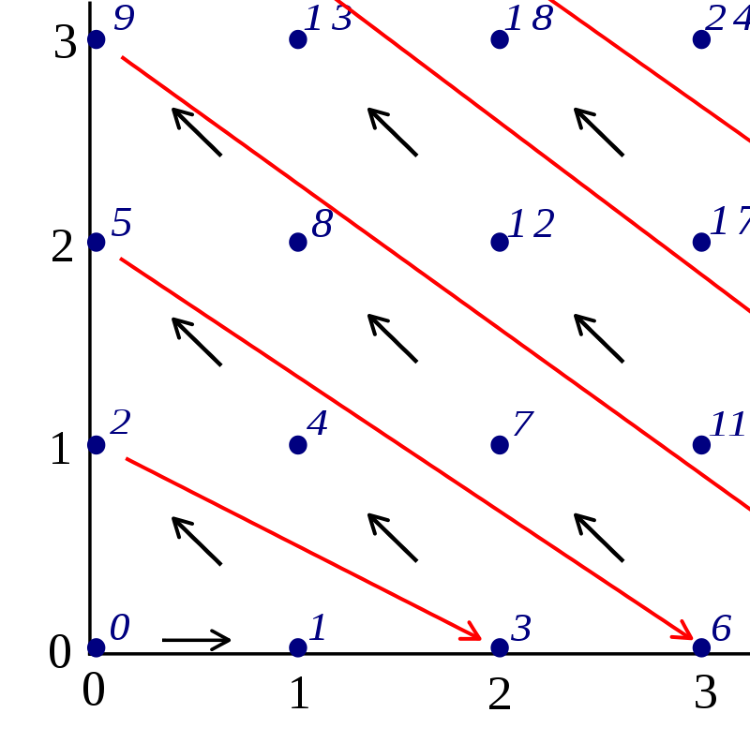
\includegraphics[width=0.5\textwidth]{Cantor.png}
	%		\caption{Cantor's pairing function}
			\label{fig:cantor}
		\end{figure}
		\item Let $f: (0,1) \rightarrow \mathbb{R}$,
		$$
		f(x)= \tan \left[ \pi \left( x-\dfrac{1}{2} \right) \right] 
		$$
		\item Let $f: [0,1] \rightarrow (0,1)$,
		$$
		f(x)= \begin{cases}\dfrac{1}{2}, & x=0 \\\dfrac{1}{n+2}, & x=1 / n, n \in \mathbb{N}\backslash \! \{0\} \\ x, & \text {otherwise}\end{cases}
		$$
	\end{enumerate}
\section{Partial Order}
\subsection{Exercise}
	1. A relation $R$ is defined on ordered pairs of integers as follows: $(x,y) R(u,v)$ if $x < u$ and $y > v$. Then $R$ is:
	\begin{enumerate}[(A)]
		\item Neither a partial order nor an equivalence relation
		\item A partial order but not a total order
		\item A total order
		\item An equivalence relation
	\end{enumerate}
	\par 
	2. Consider the set $S=\{a, b, c, d\} .$ Consider the following 4 partitions $\pi_{1}, \pi_{2}, \pi_{3}, \pi_{4}$ on $S: \pi_{1}=\{\overline{a b c d}\}, \pi_{2}=\{\overline{a b}, \overline{c d}\}, \pi_{3}=\{\overline{a b c}, \bar{d}\}, \pi_{4}=\{\bar{a}, \bar{b}, \bar{c}, \bar{d}\} .$ Let $p$ be the partial order on the set of partitions $S^{\prime}=\left\{\pi_{1}, \pi_{2}, \pi_{3}, \pi_{4}\right\}$ defined as follows: $\pi_{i} p \pi_{j}$ if and only if $\pi_{i}$ refines $\pi_{j}$ (assume the refinement relation is strict partial order here). Find the poset diagram for $\left(S^{\prime}, p\right)$. 
\subsection{Solution}
	1.  
	
	As given in question, a relation $R$ is defined on ordered pairs of integers as follows: 
	\begin{center}
		$(x,y) R(u,v)$ if $x < u$ and $y > v$,
	\end{center}  reflexive property is not satisfied here, because there is $>$ or $<$ relationship between $(x ,y)$ pair set and $(u,v)$ pair set . 
	\par Other way, if there would have been $x \leqslant u$ and $y \geqslant v$ (or $x=u$ and $y=v$) kind of relation among elements of sets then reflexive property could have been satisfied. 
	\par Since reflexive property in not satisfied here, so given relation can not be equivalence, partial order total order relation.
	\par So, option (A) is correct.
	\par 
	2. 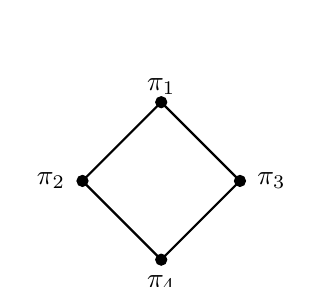
\begin{tikzpicture}
		% vertices
		\draw[fill=black] (0,1) circle (2pt);
		\draw[fill=black] (1,0) circle (2pt);
		\draw[fill=black] (1,2) circle (2pt);
		\draw[fill=black] (2,1) circle (2pt);
		% vertex labels
		\node at (-0.4,1) {$\pi_{2}$};
		\node at (1,-0.3) {$\pi_{4}$};
		\node at (1,2.2) {$\pi_{1}$};
		\node at (2.4,1) {$\pi_{3}$};
		% edges
		\draw[thick] (0,1) -- (1,0) -- (2,1) -- (1,2) -- (0,1);
		\end{tikzpicture}
		\par A partition is said to refine another partition if it splits the sets in the second partition to a larger number of sets.
		\par Therefore, the partial order contains the following ordered pairs: $$\{(\pi_4,\pi_1),(\pi_4,\pi_2),(\pi_4,\pi_3),(\pi_3,\pi_1),(\pi_2,\pi_1)\}$$
\section{Pigeonhole Principle}
\subsection{Exercise}
	1. Consider a sequence $\left\lbrace \sqrt{3}, 2\sqrt{3}, 3\sqrt{3}, \cdots \right\rbrace$ Prove that there are infinite number of terms have a mantissa of less than 0.01.
\subsection{Solution}
	\begin{proof}
		\par We represent $\left\lbrace x \right\rbrace$ as the decimal part of $x$ (\textit{e.g.}, $\left\lbrace \sqrt{3} \right\rbrace = 0.732\cdots$).
		\par  - 100 holes: $\left[ 0,0.01\right)$, $\left[ 0.01,0.02\right)$, $\cdots$, $\left[ 0.99,1\right)$.
		\par - 101 pigeons: $\left\lbrace \sqrt{3} \right\rbrace$, $\left\lbrace 2\sqrt{3} \right\rbrace$, $\cdots$, $\left\lbrace 101\sqrt{3} \right\rbrace$.
		\par $\exists m,n \in \left\lbrace 1,2,\cdots,101 \right\rbrace$, $m < n$, \textit{s.t.} $\left\lbrace m\sqrt{3} \right\rbrace$, $\left\lbrace n\sqrt{3} \right\rbrace$ belong to the same hole. Then, we have 
		\begin{itemize}
			\item Either $\left\lbrace (n-m)\sqrt{3} \right\rbrace \in \left[ 0, 0.01\right) $,
			\item or $\left\lbrace (n-m)\sqrt{3} \right\rbrace \in \left( 0.99, 1\right) $.
		\end{itemize}
		\par If $\left\lbrace (n-m)\sqrt{3} \right\rbrace \in \left[ 0, 0.01\right) $, we are done.
		\par If $\left\lbrace (n-m)\sqrt{3} \right\rbrace \in \left( 0.99, 1\right) $, represent $(n-m) \sqrt{3} = \lceil  (n-m)\sqrt{3} \rceil  - t, t \in (0,0.01)$.
		\par $\lfloor \frac{1}{t} \rfloor \cdot (n-m) \sqrt{3} = \lfloor \frac{1}{t} \rfloor \cdot \lceil (n-m) \sqrt{3} \rceil - \lfloor \frac{1}{t} \rfloor \cdot t$
		\par $\Rightarrow \left\lbrace \lfloor \frac{1}{t}\rfloor \cdot (n-m)\sqrt{3} \right\rbrace = 1 - \lfloor \frac{1}{t}\rfloor \cdot t$. Denote it as $A$.
		\par $A > 1 - \frac{1}{t} \cdot t = 0$;
		\par $A < 1 - \left( \frac{1}{t} - 1 \right) \cdot t = t < 0.01$.
		\par Therefore, $\lfloor \frac{1}{t} \rfloor (n-m) \sqrt{3}$ have a mantissa of less than 0.01.
	\end{proof}

	\section{Euclidean Algorithm}
	\subsection{Exericse}
	1. Let $F_n$ be Fermat Primes, i.e. $F_n=2^{2^n} +1$. Prove that they are 
    pairwise coprime, namely $\gcd(F_n,F_m)=1.$
    \par 
    2. Use the \textbf{Euclidean Algorithm} to find a integer pair $(x,y)$ that 
    $111x-321y=75.$ 
	\subsection{Solution}
	1. Just assume that $n>m$, let $n = m+k$, we have
	\begin{equation*}
		\begin{aligned}
			F_m &= 2^{2^m}+1 \\
			F_{m+k} & = 2^{2^{m+k}}+1 = 2^{2^m \cdot 2^k}+1
		\end{aligned}
	\end{equation*}
	So 
	$$
		F_{m+k}-2 = 2^{2^m \cdot 2^k} -1 = (2^{2^m})^{2^k}-1
	$$
	Since 
	$$
		2^{2^m} + 1 \mid (2^{2^m}) ^ {2^k} -1 \Rarrow F_m \mid F_{m+k} -2
	$$
	Considering $F_n,F_m$ are odd numbers, so $\gcd(F_n,F_m)=1$.
	\par 
	2. This is a really boring quesion, but this is highly likely to appear
	in the exam.
	\begin{itemize}
		\item Step 1. $\gcd(111,321) = 3$, so we reduce the equation to $37 x - 107 y = 25$. We first 
		solve $37x-107y=1$.
		\item Step 2. Apply the algorithm 
			\begin{equation*}
				\begin{aligned}
					107 &= 37 \times 2 + 33 \\
					37  &= 33 \times 1 + 4  \\
					33  &= 4  \times 8 + 1  \\	
					4   &= 1  \times 4
				\end{aligned}
			\end{equation*}
			So 
			\begin{equation*}
				\begin{aligned}
					1 &= 33 \times 1 - 4 \times 8 \\ 
					  &= 33 \times 1 - (37 - 33 \times 1) \times 8 \\
					  &= 37 \times (-8) + 33 \times 9 \\
					  &= 37 \times (-8) + (107-37 \times 2) \times 9 \\
					  &= 107 \times 9 + 37 \times (-26)
				\end{aligned}
			\end{equation*}
			One solution for $37x-107y=1$ is given as $(x,y)=(-26,-9)$, 
			so the solution for $37x-107=25$ can be $(x,y) = (-650,-225)$.
	\end{itemize}
	\section{Group Theory}
		\subsection{Exercise}
		1. $\mathbb{Z}^2 = \mathbb{Z} \times \mathbb{Z}$ denotes the set of pairs of integers:
		 	$$ \mathbb{Z}^2 = \{(m, n) \mid m, n \in \mathbb{Z}\}.$$ It is a group under ``vector addition'', 
		 	that is, $$(a, b) + (c, d) = (a + c, b + d).$$ Consider the set $$H = \{(x, y) \mid x + y \geqslant 0\}.$$ 
		 	Check if $H$ is a subgroup of $\mathbb{Z}^2$.
		\par \vv
		2. \begin{itemize}
			\item Can an abelian group have a non-abelian subgroup?
			\item Can a non-abelian group have an abelian subgroup?
			\item Can a non-abelian group have a non-abelian subgroup?
		\end{itemize}
		\par 
		\vv 
		3. Prove that 
		\begin{itemize}
			\item $S_n$ is non-Abelian for $n \geqslant 3$;
			\item $A_n$ is a subgroup of $S_n$;
			\item  $|A_n| = \dfrac{n!}{2}$.
		\end{itemize}
		\par \vv 
		4. Prove: For any subgroup $H \leq G$, the (left) cosets of $H$ partition the group $G$.
		\subsection{Solution}
		1. \begin{itemize}
			\item[-] Associativity: 
			\par Suppose $(a, b),(c, d),(e,f) \in H$, then $$\left[ (a, b)+(c, d)\right]  +(e,f) = (a, b)+\left[ (c, d)+(e,f)\right] = (a+c+e,b+d+f).$$
			\item[-] Closure:
			\par Suppose $(a, b),(c, d) \in H$. This means $$a + b \geqslant 0\text{ and }c + d \geqslant 0.$$ Then $$(a + c) + (b + d) = (a + b) + (c + d) \geqslant 0 + 0 = 0.$$ Therefore, $$(a, b) + (c, d) = (a + c, b + d) \in H.$$ Thus, $H$ is closed under addition.
			\item[-] Identity:
			\par Since $0 + 0 = 0 \geqslant 0$, I have $(0, 0) \in H$.
			\item[-] Inverses: 
			\par $(1, 2) \in H$, because $1 + 2 = 3 \geqslant 0$. But $−(1, 2) = (−1, −2) \notin H$, because $$−1 + (−2) = −3 \not\geqslant 0.$$ Thus, the inverse axiom fails.
		\end{itemize}
		\par Hence, $H$ is not a subgroup of $G$.
		\par \vv 
		2. No; Yes; Yes. \begin{itemize}
			\item Every subgroup of an abelian group is abelian. If $G$ is an abelian group and $H$ is a subgroup of $G$, then the operation on $H$ is commutative because it is already commutative in $G$ and $H$ is a subset of $G$. Hence an abelian group cannot have a non-abelian subgroup.
			\item A non-abelian group can have an abelian subgroup. For example, the symmetric group $S_3$ of permutation of degree 3 is non-abelian while its subgroup $A_3$ is abelian.
			\item A non-abelian group can have a non-abelian subgroup. For example, $S_4$ is a non-abelian group and its subgroup $A_4$ is also non-abelian.
		\end{itemize}
		\par \vv 
		3. \begin{enumerate}
			\item[(-)] All that we need to do here is to find two permutations $\sigma$ and $\tau$ in $S_n$ with $n \geqslant 3$ such that $\sigma \tau \neq \tau \sigma$. Indeed, consider the permutations
			$$
			\sigma=\left(\begin{array}{ccccccc}
			1 & 2 & 3 & 4 & 5 & \cdots & n \\
			1 & 3 & 2 & 4 & 5 & \cdots & n
			\end{array}\right) \quad \text { and } \quad \tau=\left(\begin{array}{ccccccc}
			1 & 2 & 3 & 4 & 5 & \cdots & n \\
			3 & 2 & 1 & 4 & 5 & \cdots & n
			\end{array}\right).
			$$
			\par Then,
			$$
			\sigma\tau=\left(\begin{array}{ccccccc}
			1 & 2 & 3 & 4 & 5 & \cdots & n \\
			2 & 3 & 1 & 4 & 5 & \cdots & n
			\end{array}\right) \quad \text { and } \quad \tau \sigma=\left(\begin{array}{ccccccc}
			1 & 2 & 3 & 4 & 5 & \cdots & n \\
			3 & 1 & 2 & 4 & 5 & \cdots & n
			\end{array}\right),
			$$
			so that $\sigma\tau \neq \tau\sigma.$
			\item[(-)] Obviously, $A_n$ is a subset of $S_n$. We then show it is a subgroup.
			\begin{enumerate}
				\item Associativity:  $\forall x,y,z \in A_n \subset S_n$, since $S_n$ is a group, $(xy)z = x(yz)$.
				\item Closure: Since the sum of two even number is even, the composition of two even bijections is even.
				\item Identity: $1 = (1) = (01)(01)$ is even, so $1 = (1) \in A_n$.
				\item Inverse: $\forall x \in A_n$, $\exists x^{-1} \in S_n$ is also in $A_n$ because it has the same number of transportation as $x$, which is even. 
			\end{enumerate}
			\par Therefore, $A_n$ is a subgroup of $S_n$.
			\item[(-)] Denote the set of all odd permutations in $S_n$ as $B_n$. We aim to prove $|A_n| = |B_n|$, \textit{i.e.}, there exists a bijection between $A_n$ and $B_n$. Demote this bijection by $F$, and we have $F: A_n \to B_n$. Let $F(\sigma) = (01)\sigma$, where $\sigma \in A_n$ is even.
			\begin{enumerate}
				\item Injection: Assume $\sigma_1, \sigma_2 \in A_n$. If $\sigma_1 \neq \sigma_2$,  $(01)\sigma_1 \neq (01)\sigma_2$. Therefore, $F$ is injective.
				\item Surjection: Every $\tau_1 \in B_n$ can be represented as $(01)\tau_2$ where $\tau_2 \in A_n$ because $\tau_1 = (01)\tau_2 = (01)(01)\tau_1$ where $\tau_2 = (01)\tau_1$ is even. Hence $F$ is surjective.
			\end{enumerate}
			\par Therefore, $F$ is a bijection. Considering $|S_n| = n!$, we have $|A_n| = \dfrac{n!}{2}$.
			\end{enumerate}
		\par \vv 
		4. We need to show that the union of the left cosets is the whole group, and that different cosets do not overlap. 
		\begin{itemize}
			\item For all $g \in G$, $g \in gH$ since $H$ is a subgroup of $G$ which includes the identity $1_G$. . This shows that every element of $G$ lies in some coset of $H$, so the union of the cosets is all of $G$.
			\item Suppose $a H$ and $b H$ are two cosets of $H$, and suppose they are not disjoint. We must show they are identical: $a H = b H$ . As usual, we can show two sets are equal by showing that each is contained in the other.
			\par Since $a H$ and $b H$ are not disjoint, we can find an element $g \in a H \cap b H$ . Write $g = a h_1 = b h_2$ for $h_1, h_2 \in H$ . Then $$a = b h_2 h_1^{-1}.$$
			\par Now let $a h \in aH$ . Then	$$a h = b h_2 h_1^{-1} h.$$
			\par The element on the right is in $b H$ , since it is $b$ times$ h_2 h_1^{-1} h \in H$. Therefore, $a h \in b H$, \textit{i.e.}, $a H \subset b H$ . By symmetry, $b H \subset a H$, so $a H = b H$.
		\end{itemize}
	\section{Graph Theory}
		\subsection{Exercise}
		1. The complement of a simple graph $G = (V, E)$ is given by 
		$G\,^c = (V, E\,^c)$, where $E\,^c = V \times V ~\cut~ E$, i.e., the
    	complement has the same vertex set and an edge is in $E\,^c$
    	if and only if it is not in $E$. A graph $G$ is said to be
    	\blue{\textit{self-complementary}} if $G$ is isomorphic to $G\,^c$.
    	\begin{itemize}
    	    \item[i)] Show that a self-complementary graph must have either $4m$ or $4m + 1$ vertices, $m\in\bN$.
    	    \item[ii)] Find all self-complementary graphs with 8 or fewer vertices.
    	\end{itemize}
    	(Taken from Ve203 FA2020 Assignment10)
		\subsection{Solution}
		1. \par \vspace{1em}
		\hh i) Consider $G \cup G\,^c = \(V,E\cup E\,^c \) = K_n$, there are 
		in total $\binom{n}{2}$ edges. The total number of edges must be even.
		We consider the remainder of $n$ modulo $4$: 
		\begin{itemize}
			\item $n = 4m $: $$\binom{4m}{2} = \frac{4m(4m-1)}{2} = 2m\cdot (4m-1) \text{  ~~~- even }\surd$$
			\item $n = 4m+1 $: $$\binom{4m+1}{2} = \frac{4m(4m+1)}{2} = 2m \cdot (4m+1)  \text{  ~~~- even }\surd$$
			\item $n = 4m+2 $: $$\binom{4m+2}{2} = \frac{(4m+1)(4m+2)}{2} = (2m+1) \cdot (4m+1)  \text{  ~~~- odd~ }\times$$
			\item $n = 4m+3 $: $$\binom{4m+3}{2} = \frac{(4m+3)(4m+2)}{2} = (2m+1) \cdot (4m+3)   \text{  ~~~- odd~ }\times$$
		\end{itemize}
		\par 
		\hh ii) $n$ can only be $4$ or $5$. Consider $C_5$ and $P_4$.
		
\end{document}